\documentclass{article} % For LaTeX2e
\usepackage{nips15submit_e,times}
\usepackage{hyperref}
\usepackage{url}
%\documentstyle[nips14submit_09,times,art10]{article} % For LaTeX 2.09
\usepackage{graphicx} % add this in the preamble
\usepackage{amssymb}
\usepackage{amsthm}
\usepackage{amssymb}
\usepackage{amsthm}
\usepackage{amsmath}	
\usepackage{amsfonts}
\usepackage{amsopn}
\usepackage{bm}

\usepackage{lineno}
\usepackage{graphicx} 
\usepackage{booktabs} 
\usepackage{epsfig}
\usepackage{hyperref}
\usepackage{lipsum}
\usepackage{mathtools}
\usepackage{xspace}
\usepackage{array}
\usepackage{multirow}
\usepackage{enumerate}
\usepackage{rotating}
\usepackage{caption} 
\usepackage{subcaption}
\usepackage{listings}
\usepackage{natbib}
\usepackage{comment}
\usepackage{pdflscape}
\usepackage{breqn}
\usepackage{float}

\title{Deep learning for topology optimization}


\author{
Sy Nguyen-Van \\
School of Mechanical, Aerospace, and Manufacturing Engineering\\
University of Connectivcut\\
Storrs, CT 06269 \\
\texttt{sy.nguyen-van@uconn.edu} \\
}

% The \author macro works with any number of authors. There are two commands
% used to separate the names and addresses of multiple authors: \And and \AND.
%
% Using \And between authors leaves it to \LaTeX{} to determine where to break
% the lines. Using \AND forces a linebreak at that point. So, if \LaTeX{}
% puts 3 of 4 authors names on the first line, and the last on the second
% line, try using \AND instead of \And before the third author name.

\newcommand{\fix}{\marginpar{FIX}}
\newcommand{\new}{\marginpar{NEW}}

\nipsfinalcopy % Uncomment for camera-ready version

\begin{document}


\maketitle

\begin{abstract}
In mechanical engineering, design problems often involve minimizing weight while maximizing mechanical performance. One of the most effective approaches to achieve this is topology optimization, which determines the optimal material distribution within a given design domain. However, traditional topology optimization faces two main challenges: computationally expensive finite element simulations and error-prone gradient calculations. To address these issues, this proposal aims to leverage deep learning as an alternative to conventional topology optimization in mechanical engineering.
\end{abstract}

\section{Introduction}
In mechanical engineering, to optimize the mechanical structures, we usually use topology optimization. This method essentially find the optimal material distribution within the design domain and simultaneously maximize mechanical performance such as stiffness, strength. 

For instance, Fig.~\ref{Fig_Lbracket2d}.a illustrates the initial design, consisting of a frame with the left side fixed and the right side supported by rollers, subjected to a compressive load. The objective is to maximize structural stiffness while constraining the volume fraction in order to reduce the mass. In topology optimization, we discrete the domain into finite element or voxel as show in Fig.\Ref{Fig_Lbracket2d_Mesh}.

The next step is to compute the analytical gradients of the objective and constraint functions with respect to the density of each voxel, and then apply a gradient-based optimizer to automatically find the optimal solution.

% -----------------------------------
\begin{figure}[H] 
	\centering
	\begin{subfigure}{0.4\textwidth} \centering
		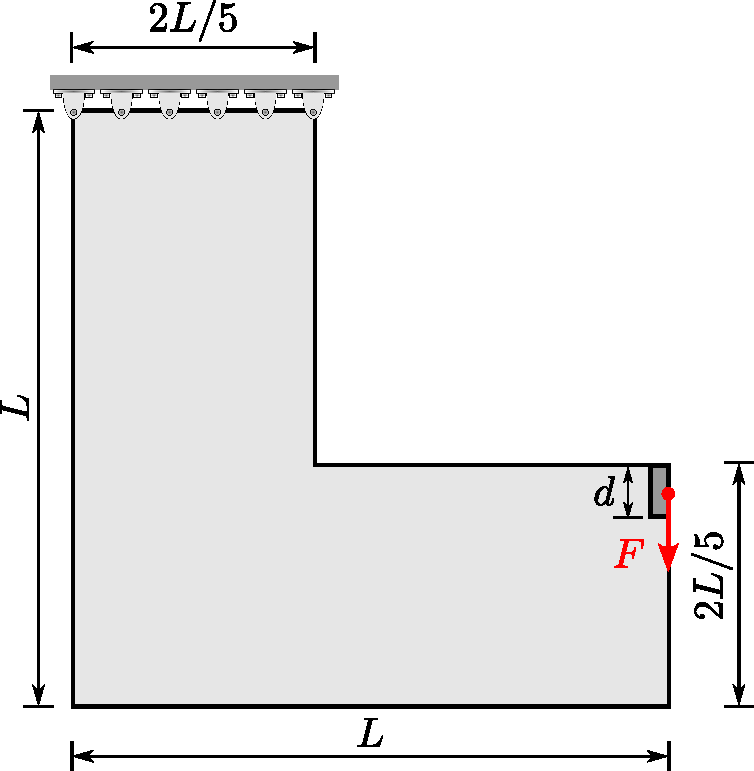
\includegraphics[scale=0.35]{Lbracket2d.pdf}
		\caption{}
	\end{subfigure}
	% -----------------------------------
	\begin{subfigure}{0.4\textwidth} \centering
		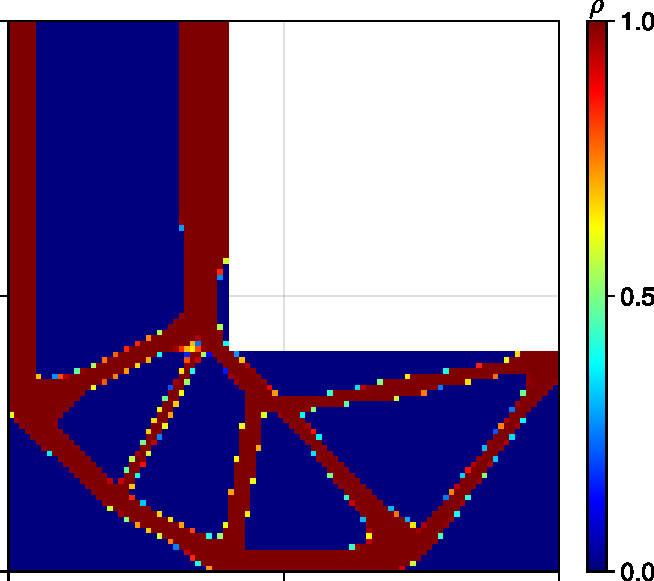
\includegraphics[scale=0.4]{Lbracket2d_TOP.pdf}
		\caption{}
	\end{subfigure}
	\caption{The initial design domain and the corresponding optimal design.}
	\label{Fig_Lbracket2d}
\end{figure}
% ------------------------------
\begin{figure}[htp!]
		\centering
		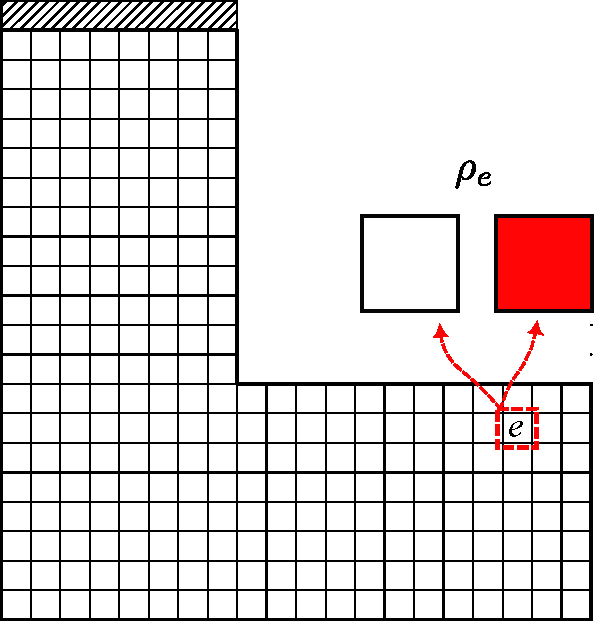
\includegraphics[scale=0.35]{TOP_Variables.pdf}
	\caption{Finite element (voxels) mesh.}
	\label{Fig_Lbracket2d_Mesh}
\end{figure}
 % ==============================
\section{Proposed method}
In topology optimization, we need to run the finite element method (FEM) to solve partial differential equations (PDEs) in order to evaluate the objective and constraint functions, which is computationally expensive for large scale problems. In addition, the derivation of gradients of functions is error-prone. 

Therefore, to overcome these issues in conventional topology optimization, a deep learning-based approach is proposed as shown in Fig.\ref{Fig_DL_TOP}.
To apply deep learning for topology optimization, the input is the initial design domain along with the boundary conditions, while the output is the corresponding optimal design. To generate the output, we still need to use topology optimization. 

After, we obtain the sufficient datasets, we could use CNN, Unet, etc to train the model. With that, with the fine tune model, we just need to give any new input to predict the optimal design without running FEM and computing the gradient of mechanical functions.

It should be noted that he proposed method should not be seen as a complete replacement for conventional topology optimization, as machine learning is limited to interpolation within the available dataset. Therefore, when applied to new structures or boundary conditions, its performance may be less reliable. Nevertheless, it can still serve as a valuable starting point before running the conventional approach.

% ------------------------------
\begin{figure}[htp!]
	\centering
	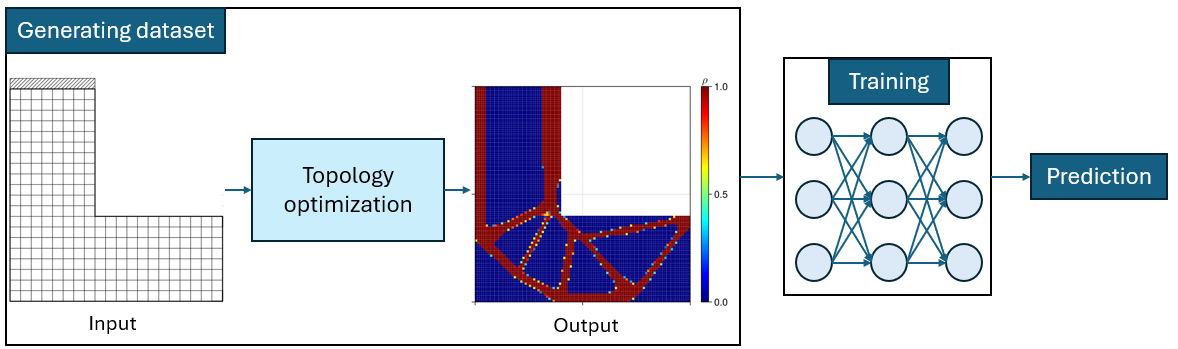
\includegraphics[scale=0.45]{DL_TOP.png}
	\caption{Flowchart of the proposed deep learning for topology optimization.}
	\label{Fig_DL_TOP}
\end{figure}

\section{Schedules}

\begin{table}[h!]
	\centering
	\caption{Research schedule from September to December 2025.}
	\label{tab:schedule}
	\begin{tabular}{|c|l|}
		\hline
		\textbf{Time Period} & \textbf{Task} \\ \hline
		Now -- 15th October   & Obtaining data \\ \hline
		15th October -- 1st November & Training deep learning models \\ \hline
		1st November -- 1st December & Getting and analyzing results \\ \hline
	\end{tabular}
\end{table}




\end{document}
